\documentclass{beamer} % Frames.
%\documentclass[notes]{beamer} % Frames and notes.
%\documentclass[notes=only]{beamer} % Notes.

\usetheme{BTH}

\usepackage{calc}
\usepackage{tikz}
\usepackage{float}
\usepackage{mdwlist}
\usepackage{multirow}
\usepackage{multicol}
\usepackage{hyperref}
\usepackage{listings}

\floatstyle{plaintop}
\restylefloat{table}

\lstset{ 
  language=C,
  tabsize=2,
  backgroundcolor=\color{black!5},
  basicstyle=\tiny,
}

\title{ACCELERATING GPU WORKLOAD SIMULATION USING MICROSOFT WARP}
\author{Eric Nilsson}
\institute{Blekinge Institute of Technology}
\date{\today}

\begin{document}
{% Don't feature a footer on the title page:
  \setbeamertemplate{footline}{} 
  \begin{frame}
    \titlepage
  \end{frame}
}

\setbeamertemplate{section in toc}{\inserttocsectionnumber.~\inserttocsection}
\setbeamertemplate{subsection in toc}{%
  \hspace{0.5cm}\rule[0.3ex]{3pt}{3pt}~\inserttocsubsection\par}

\AtBeginSection[]
{%
  \begin{frame}
    \frametitle{TABLE OF CONTENTS}
    \begin{multicols}{2}
    \tableofcontents[currentsection]
    \end{multicols}
  \end{frame}
}

\setbeamertemplate{caption}{\raggedright\insertcaption\par}

\definecolor{bth_black}{RGB}{0, 0, 0}
\setbeamercolor{section in toc}{fg=bth_black}
\setbeamercolor{block title}{fg=bth_black}

% INTRODUCTION
% GAME_HARD_01_PRESENTATION_INTRODUCTION.tex
\section{Introduction}

% GRAPHICS SIMULATION
\subsection{Graphics Simulation}
\begin{frame}
\frametitle{GRAPHICS SIMULATION}

\begin{itemize}
\item Common method of verifying GPU workloads, such as computer graphics, by eliminating dependency to third-party drivers and hardware
\item Often orders of magnitude too slow for complex applications
\end{itemize}

\end{frame}

% EXAMPLE
\subsection{Example}
\begin{frame}
\frametitle{EXAMPLE}

\begin{figure}[ht]
  \begin{minipage}[b]{0.3\linewidth}
    \centering
    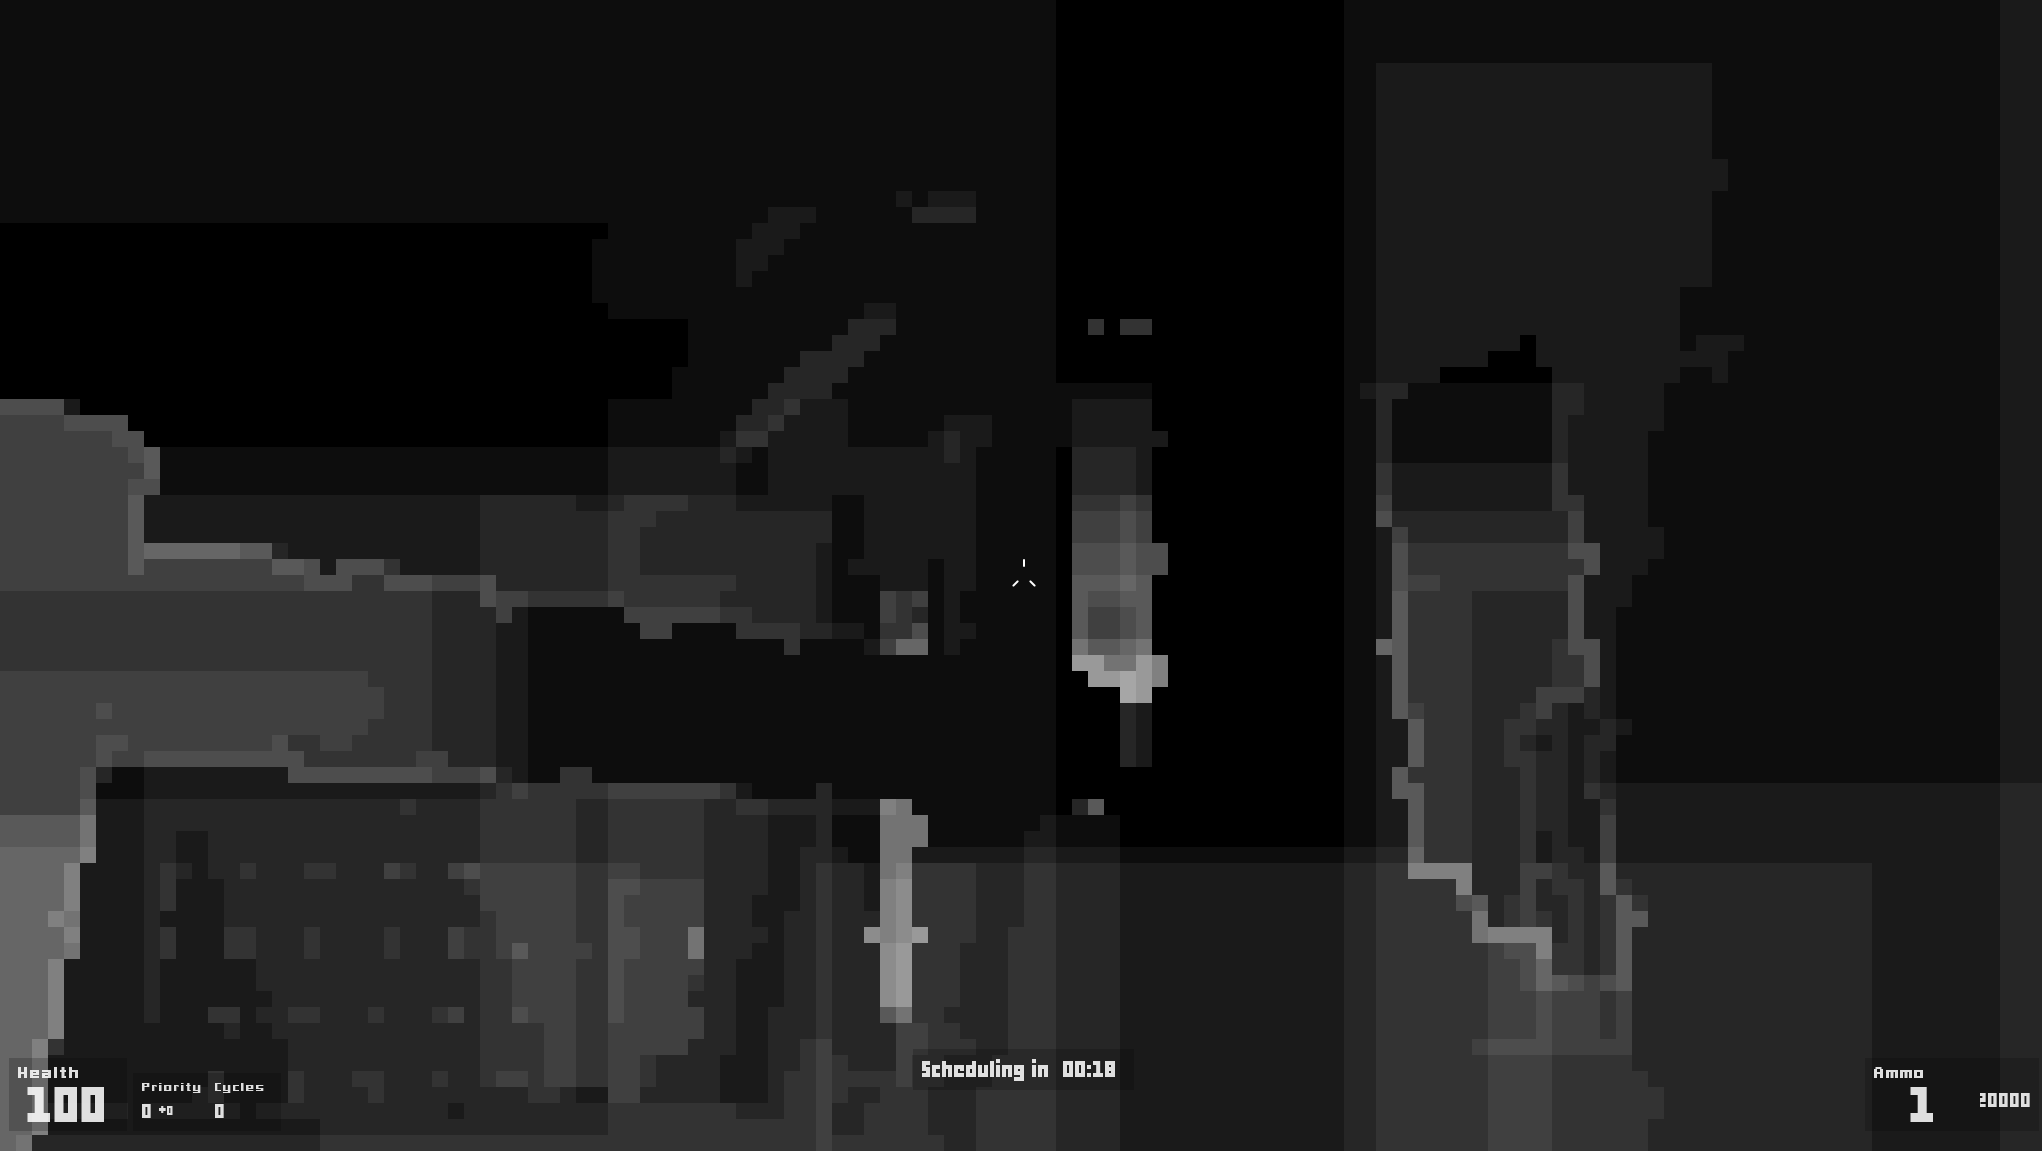
\includegraphics[width=1.0\textwidth]{img/tbds1.png}
  \end{minipage}
  \hspace{0.25cm}
  \begin{minipage}[b]{0.3\linewidth}
    \centering
    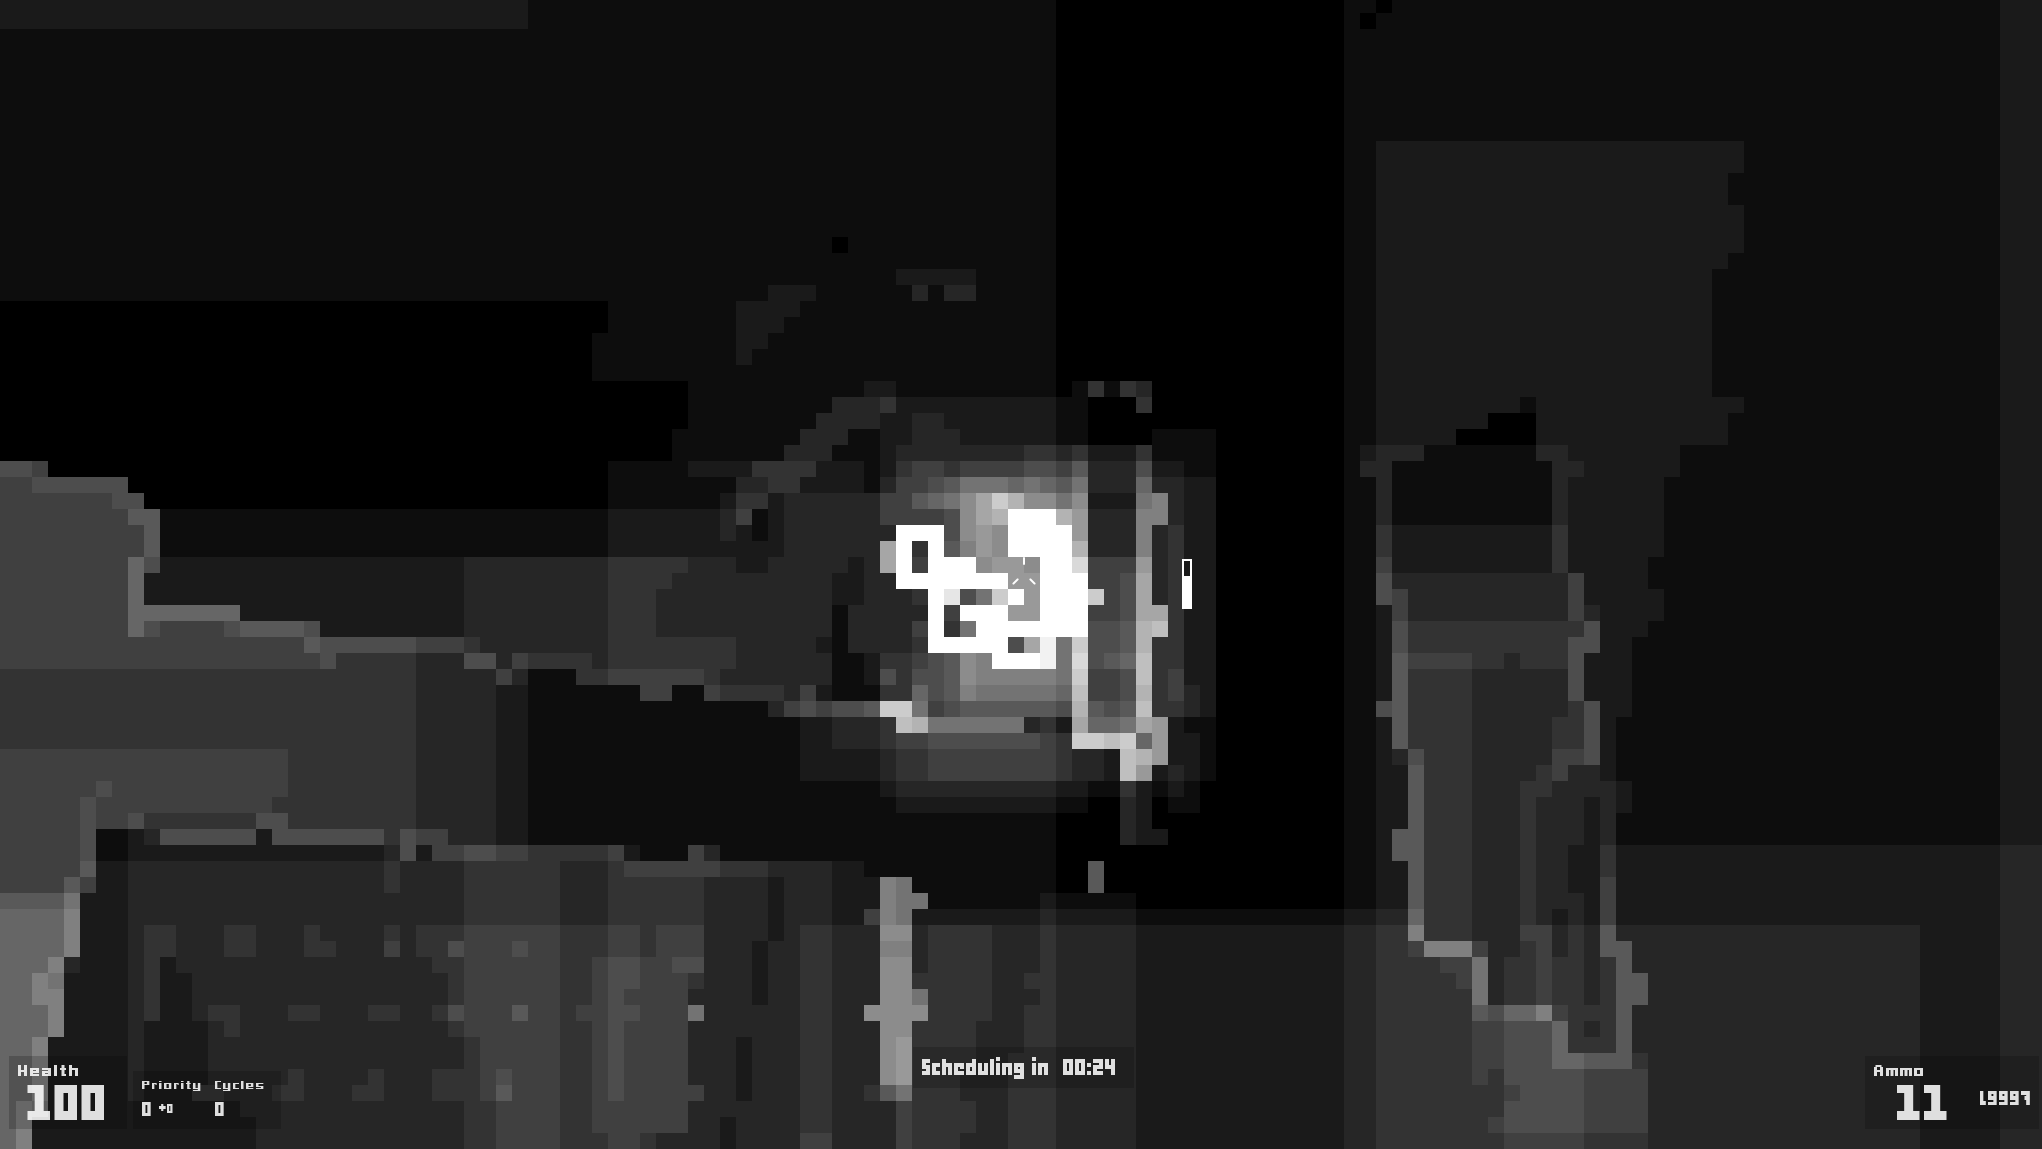
\includegraphics[width=1.0\textwidth]{img/tbds2.png}
  \end{minipage}
  \hspace{0.25cm}
  \begin{minipage}[b]{0.3\linewidth}
    \centering
    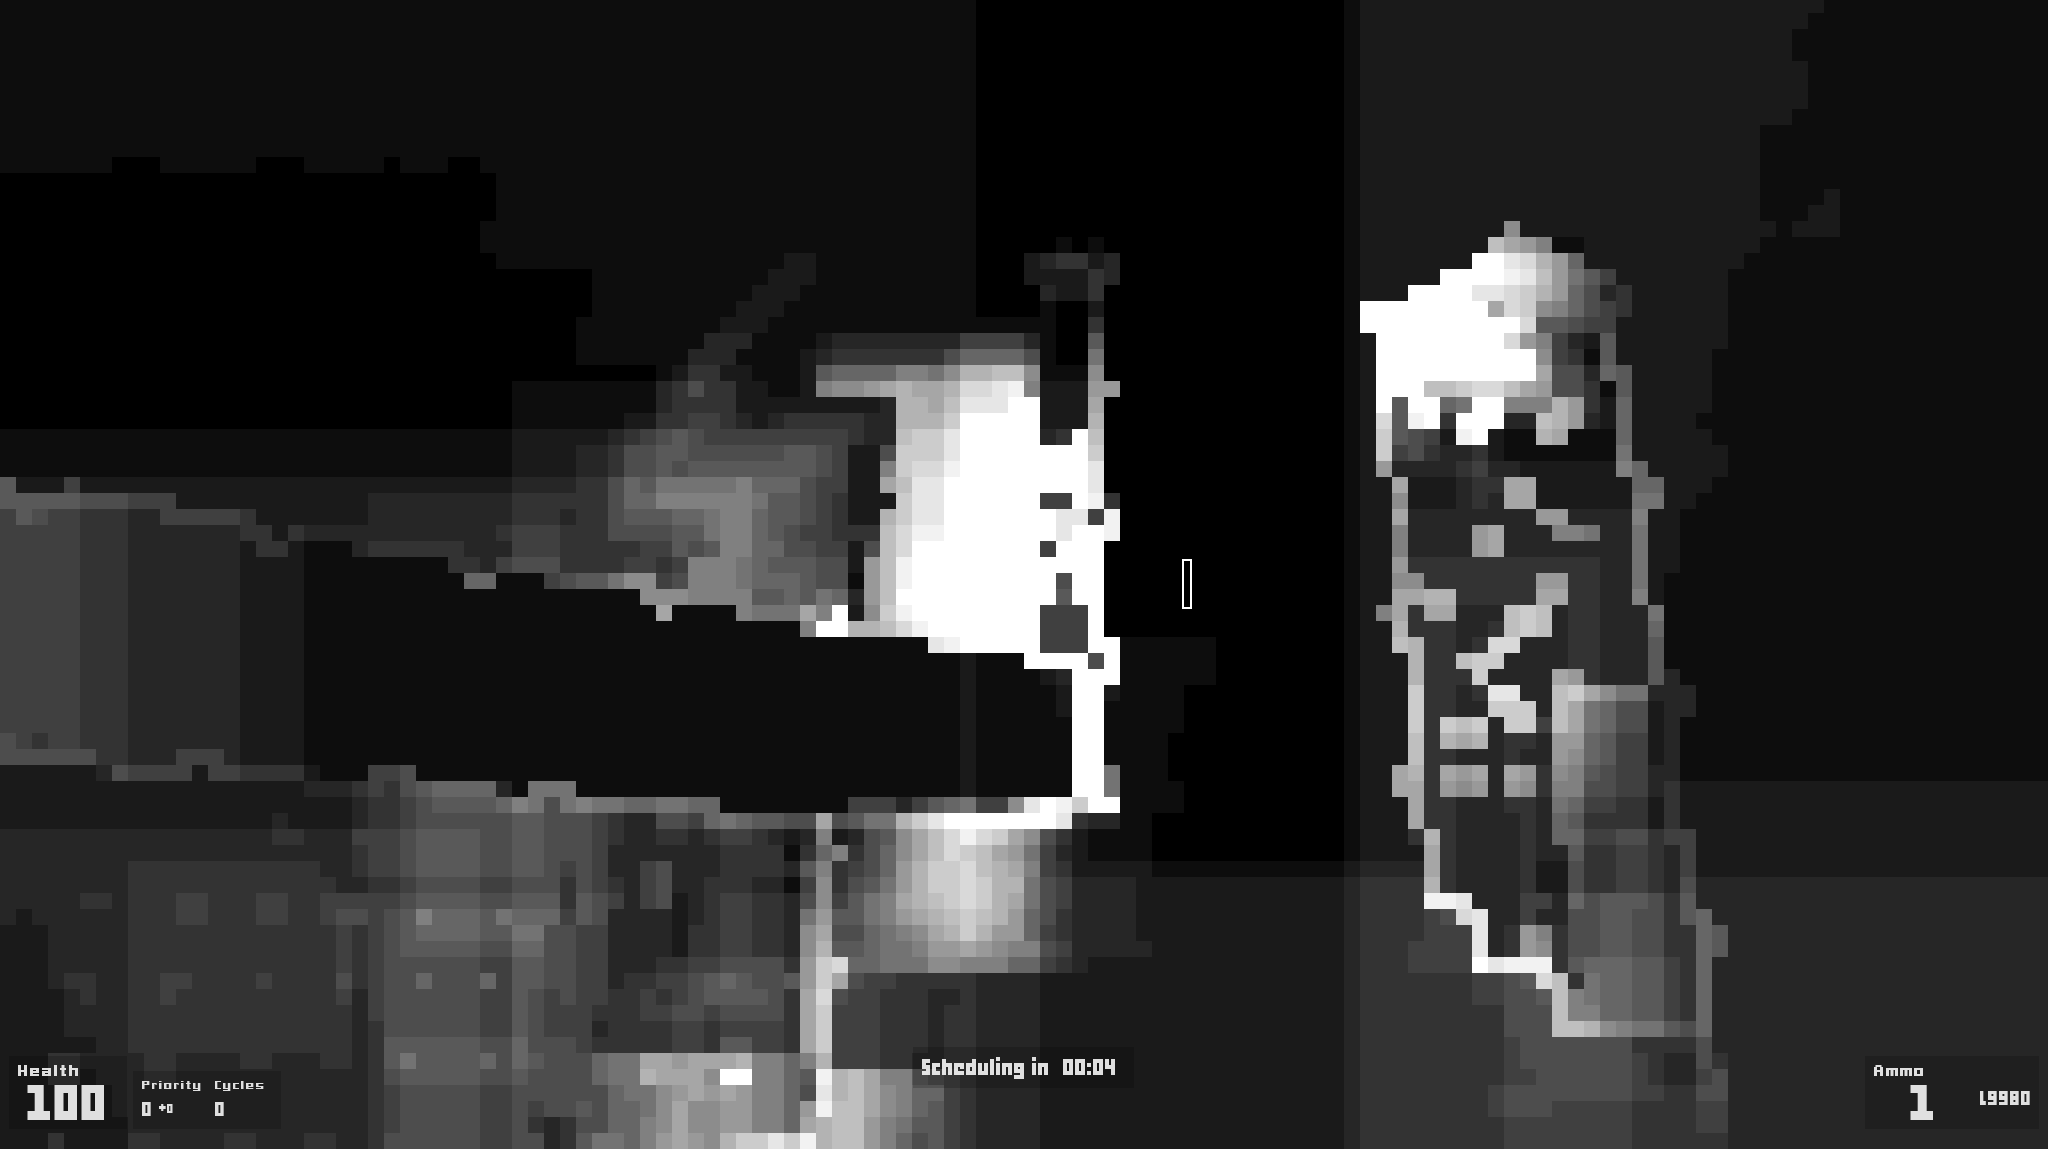
\includegraphics[width=1.0\textwidth]{img/tbds3.png}
  \end{minipage}
  \label{fig:tilingvisualization}
  \caption{Tile-based deferred shading using DirectCompute.}
\end{figure}

\begin{figure}[ht]
  \begin{minipage}[b]{0.3\linewidth}
    \centering
    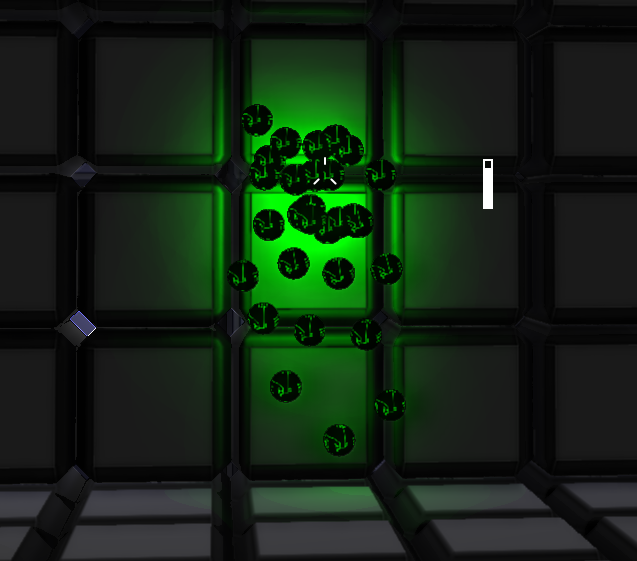
\includegraphics[width=1.0\textwidth]{img/tbds.png}
    \caption{AMD}
  \end{minipage}
  \hspace{0.25cm}
  \begin{minipage}[b]{0.3\linewidth}
    \centering
    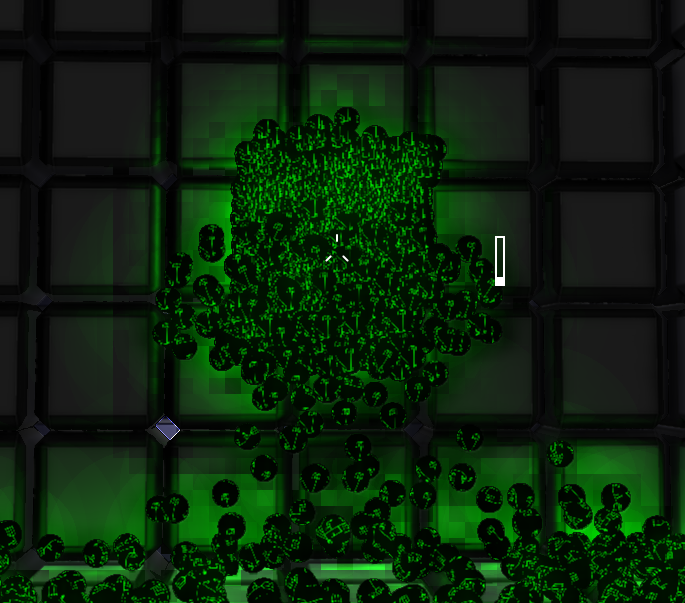
\includegraphics[width=1.0\textwidth]{img/tbds_error.png}
    \caption{NVIDIA\textit{*≠}}
  \end{minipage}
  \label{fig:tilingerror}
\end{figure}

\end{frame}

% WARP
\subsection{Microsoft WARP}
\begin{frame}
\frametitle{MICROSOFT WARP}

Introductory frame on Microsoft WARP.

\end{frame}

% CONTRIBUTION
% GAME_HARD_01_PRESENTATION_CONTRIBUTION.tex
\section{Contribution}

% EXPERIMENT
\subsection{Experiment}
\begin{frame}
\frametitle{EXPERIMENT}

$200\times 200$ matrix multiplication using Direct3D DirectCompute:

\begin{enumerate*}
\item Randomize matrices $A$ and $B$
\item Establish $AB=Ref$
\item Start high-precision timer
\item Calculate $AB=C$ using Direct3D
\item Stop high-precision timer
\item Verify $C$ and $Ref$ deviation
\end{enumerate*}

\end{frame}

% DIRECTCOMPUTE KERNELS
\subsection{DirectCompute Kernels}
\begin{frame}[t]
\frametitle{DIRECTCOMPUTE KERNELS}

\begin{columns}[T]
  \begin{column}[T]{0.5\textwidth}
    \begin{center}1.\end{center}
    Matrix mult. w. Thread Blocks:
    \begin{itemize}
    \item Invoked once per entry
    \item Performed in blocks of $16\times 16$
    \end{itemize}
  \end{column}
  \begin{column}[T]{0.5\textwidth}
    \begin{center}2.\end{center}
    Matrix mult. w. Thread Blocks and Shared Memory:
    \begin{itemize}
    \item Utilizes shared memory to cache matrices
    \end{itemize}
  \end{column}
\end{columns}

{\footnotesize\it%
  \begin{block}{}
    \begin{columns}[T]
      \begin{column}[T]{0.33\textwidth}
        Constant Memory:
        \begin{itemize}
        \item Latency- and bandwidth oriented memory
        \item Read-only device access
        \end{itemize}
      \end{column}
      \begin{column}[T]{0.33\textwidth}
        Global Memory:
        \begin{itemize}
        \item Device main memory
        \item Read- and write access by device host
        \end{itemize}
      \end{column}
      \begin{column}[T]{0.33\textwidth}
        Shared Memory:
        \begin{itemize}
        \item High-speed device read-/write memory
        \item May be accessed across 'blocks'
        \end{itemize}
      \end{column}
    \end{columns}
  \end{block}
}

\end{frame}

% TEST CASES
\subsection{Test Cases}
\begin{frame}
\frametitle{TEST CASES}

\begin{block}{1. Hardware-Acceleration}
  \begin{itemize}
  \item Execution on a modern video card
  \item Maximising FLOPS output
  \item First reference measurement for the performance of WARP
  \end{itemize}
\end{block}
\noindent\rule{11cm}{0.4pt}
\begin{block}{2. Software Rasterization}
  \begin{itemize}
  \item Traditional software rasterization using the reference device driver
  \item Second reference measurement for the performance of WARP
  \end{itemize}
\end{block}
\begin{block}{3. Windows Advanced Rasterization Platform}
  \begin{itemize}
  \item Software rendering using WARP
  \end{itemize}
\end{block}

\end{frame}

% SOFTWARE
\subsection{Software}
\begin{frame}
\frametitle{SOFTWARE}

\begin{columns}[T]
  \begin{column}{0.33\textwidth}
    \textbf{matrixgen}\hfill$\rightarrow$\hfill
    \begin{itemize}
    \item Generates $A$ \& $B$
    \item Establishes $Ref$
    \item C$++$ and $C±±$~AMP
    \end{itemize}
  \end{column}
  \begin{column}{0.33\textwidth}
    \textbf{experiment}\hfill$\rightarrow$\hfill
    \begin{itemize}
    \item Produces $C$ using Direct3D
    \item Performs $100$ tests for each scenario:
      \begin{itemize}
      \item Kernel
      \item Precision\footnotemark
      \item Acceleration
      \end{itemize}
    \item C$++$ and HLSL
    \end{itemize}
  \end{column}
  \begin{column}{0.33\textwidth}
    \textbf{analytics}
    \begin{itemize}
    \item Analyzes raw data
    \item Compiles measurement average:
      \begin{itemize}
      \item Min/Max
      \item Avg
      \item StD
      \end{itemize}
    \item C$++$
    \end{itemize}
  \end{column}
\end{columns}

\footnotetext[1]{We perform the experiment in both integer and floating point precision.}

\end{frame}

% Arrowhead command. Sets a tikz node for rendering an entire arrow.
\newcommand\ah[2]{\tikz[remember picture,baseline]\node[inner sep=2pt,outer sep=0](#1){#2};}
% Arrow command. Draws an arrow between two tikz nodes.
\newcommand\arrow[2]{%
  \begin{tikzpicture}[remember picture, overlay, >=stealth, shift={(0,0)}]
    \draw[->] (#1) to (#2);
  \end{tikzpicture}%
}

% RESULTS
\subsection{Results}
\begin{frame}
\frametitle{RESULTS}

\begin{columns}[T]
  \begin{column}{0.2\textwidth}
    \textbf{Integer precision (ms):}
  \end{column}
  \begin{column}{0.8\textwidth}
    \begin{center}
      \begin{tabular}{r|r|r|r|}
        \cline{2-3}
        & \multicolumn{1}{|c|}{1. Naïve} & \multicolumn{1}{|c|}{2. Tiled} \\ \hline
        \multicolumn{1}{|l|}{Hard}     & \ah{hh1}{$1.16$}      & \ah{hf1}{\phantom{0000}$0.24$}\ah{spc}{}      & \ah{spc}{$-79.3\%$} \\ \hline \hline
        \multicolumn{1}{|l|}{Soft}     & \ah{vh2}{}\ah{hh2}{$11610.02$}        & \ah{hf2}{\phantom{0}$9866.40$}\ah{vh1}{}      & \ah{spc}{$-15.0\%$} \\ \hline
        \multicolumn{1}{|l|}{WARP}     & \ah{vf2}{}\phantom{000}\ah{hh3}{$15.31$}      & \ah{hf3}{\phantom{000}$18.97$}\ah{vf1}{}      & \ah{spc}{$+23.9\%$} \\ \hline
        & \multicolumn{1}{|r|}{\ah{spc}{$-99.9\%$}} & \multicolumn{1}{|r|}{\ah{spc}{$-99.8\%$}} \\ \cline{2-3}
      \end{tabular}
      \arrow{hh1}{hf1} % Draw horizontal arrow heads to fletchlings.
      \arrow{hh2}{hf2}
      \arrow{hh3}{hf3}
      \arrow{vh1}{vf1} % Draw vertical arrow heads to fletchlings.
      \arrow{vh2}{vf2}
    \end{center}
  \end{column}
\end{columns}

\begin{columns}[T]
  \begin{column}{0.2\textwidth}
      \textbf{Floating point precision (ms):}
  \end{column}
  \begin{column}{0.8\textwidth}
    \begin{center}
      \begin{tabular}{r|r|r|r|}
        \cline{2-3}
        & \multicolumn{1}{|c|}{1. Naïve} & \multicolumn{1}{|c|}{2. Tiled} \\ \hline
        \multicolumn{1}{|l|}{Hard}     & \ah{hh1}{$0.77$}      & \ah{hf1}{\phantom{0000}$0.22$}\ah{spc}{}      & \ah{spc}{$-71.4\%$} \\ \hline \hline
        \multicolumn{1}{|l|}{Soft}     & \ah{vh1}{}\ah{hh2}{$10247.03$}        & \ah{hf2}{$10909.88$}\ah{vh2}{}        & \ah{spc}{$+\phantom{0}6.5\%$} \\ \hline
        \multicolumn{1}{|l|}{WARP}     & \ah{vf1}{}\phantom{000}\ah{hh3}{$14.08$}      & \ah{hf3}{\phantom{000}$17.44$}\ah{vf2}{}      & \ah{spc}{$+23.9\%$} \\ \hline
        & \multicolumn{1}{|r|}{\ah{spc}{$-99.9\%$}} & \multicolumn{1}{|r|}{\ah{spc}{$-99.8\%$}} \\ \cline{2-3}
      \end{tabular}
      \arrow{hh1}{hf1} % Draw horizontal arrow heads to fletchlings.
      \arrow{hh2}{hf2}
      \arrow{hh3}{hf3}
      \arrow{vh1}{vf1} % Draw vertical arrow heads to fletchlings.
      \arrow{vh2}{vf2}
    \end{center}
  \end{column}
\end{columns}

\end{frame}

% SHARED MEMORY IMPACT
\subsection{Shared Memory Impact}
\begin{frame}
\frametitle{SHARED MEMORY IMPACT}

\begin{center}
\resizebox{\columnwidth}{!}{\input{../msswarp}}
\end{center}

\end{frame}

% CONCLUSION
% GAME_HARD_01_PRESENTATION_CONCLUSION.tex
\section{Conclusion}

% SUBSECTION
\subsection{Subsection}
\begin{frame}
\frametitle{SUBSECTION}

\end{frame}

% GAME_HARD_01_PRESENTATION_CLOSING.tex

\begin{frame}
\frametitle{}

\begin{center}
Source code and raw data available for download:
\url{http://bit.ly/MicrosoftWARP}
\end{center}

\end{frame}

% Closing frame:
% Source code and data available
% May be downloaded if you want to replicate the test
 % Closing frame.
% APPENDIX
% GAME_HARD_01_PRESENTATION_APPENDIX.tex
\section{Appendix}

% DIRECTCOMPUTE KERNELS
\subsection{DirectCompute Kernels}
\begin{frame}[fragile]
\frametitle{DIRECTCOMPUTE KERNELS}

\begin{multicols}{2}
\begin{lstlisting}
[numthreads(BLOCK_SIZE, BLOCK_SIZE, 1)]
void main(
  uint3 tIdx : SV_GroupThreadID,
  uint3 bIdx : SV_GroupID){
  const uint row =
    bIdx.y*BLOCK_SIZE+tIdx.y;
  const uint col =
    bIdx.x*BLOCK_SIZE+tIdx.x;
  if(row>=cRows || col>=cCols){
    return;
  }

  float sum = 0;
  for(uint i = 0; i<aRows; i++){
    uint idxA = row*aRows+i;
    uint idxB = col+bRows*i;
    sum += mA[idxA]*mB[idxB];
  }
  mC[row*cRows+col] = sum;
}
\end{lstlisting}
\begin{lstlisting}
groupshared float mAs
  [BLOCK_SIZE][BLOCK_SIZE];
groupshared float mBs
  [BLOCK_SIZE][BLOCK_SIZE];

[numthreads(BLOCK_SIZE, BLOCK_SIZE, 1)]
void main(
  uint3 tIdx : SV_GroupThreadID,
  uint3 bIdx : SV_GroupID){
  const uint row = bIdx.y
    *BLOCK_SIZE+tIdx.y;
  const uint col = bIdx.x
    *BLOCK_SIZE+tIdx.x;
  
  float sum = 0;
  const uint blocks = ceil( 
    (float)aRows/(float)BLOCK_SIZE);
  for(uint i = 0; i<blocks; i++){
    mAs[tIdx.y][tIdx.x] = mA[ 
      row*aRows+(i*BLOCK_SIZE+tIdx.x)];
    mBs[tIdx.y][tIdx.x] = mB[ 
      col+bRows*(i*BLOCK_SIZE+tIdx.y)];
    GroupMemoryBarrierWithGroupSync();

    for(uint j = 0; j<BLOCK_SIZE; j++){
      sum += 
        mAs[tIdx.y][j]*mBs[j][tIdx.x];
    }
    GroupMemoryBarrierWithGroupSync();
  }
  if(row>=cRows || col>=cCols){
    return;
  }
  mC[row*cRows+col] = sum;
}
\end{lstlisting}
\end{multicols}

\end{frame}


\end{document}
